\documentclass[utf8x]{beamer}

\mode<presentation>
{
  \usetheme{Warsaw}

  %\setbeamercovered{transparent}
}

\usepackage[english]{babel}

\usepackage[utf8x]{inputenc}

\usepackage{times}
\usepackage[T1]{fontenc}

\title{The speed of PyPy}

\author{Maciej Fijałkowski}

\institute[merlinux GmbH]
{ merlinux GmbH }

\date{RuPy, November 7th 2009, Poznań}

\begin{document}

\begin{frame}
  \titlepage
\end{frame}

\begin{frame}

  \frametitle{Story about Python's speed}
  \begin{figure}
    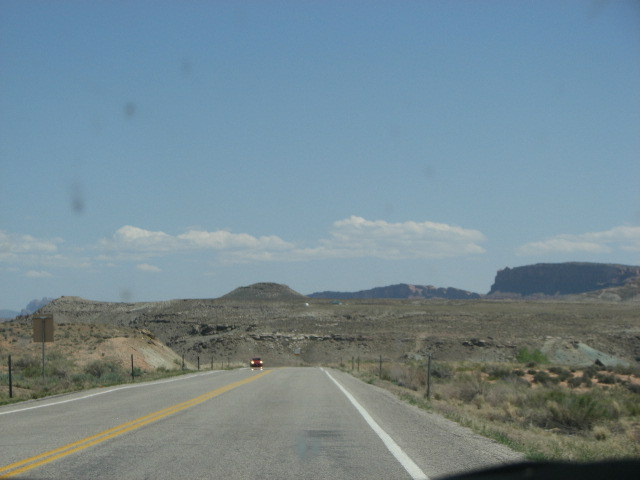
\includegraphics[width=.8\textwidth]{img1.jpg}
  \end{figure}

\end{frame}

\begin{frame}
  \frametitle{Speed of Python}
  \begin{itemize}
     \item Python is slow
  \end{itemize}
  \pause
  \begin{figure}
    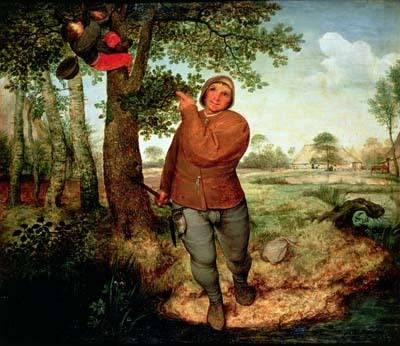
\includegraphics[width=.6\textwidth]{peasant_and_birdnester-400.jpg}
  \end{figure}
  
\end{frame}

\begin{frame}
  \frametitle{Speed of Python}
  \begin{itemize}
    \item Is Python really slow?
      \pause
    \item Sometimes
      \pause
    \item Let's have a look at some examples
  \end{itemize}

\end{frame}

\begin{frame}
  \frametitle{Nomenclature}
  \begin{itemize}
    \item Python - a programming language
    \item CPython - main implementation of Python
    \item JVM - Java Virtual Machine - VM used to run Java, among others
    \item JIT - Just in time compiler
    \item Psyco - JIT for Python
  \end{itemize}
\end{frame}

\begin{frame}
  \frametitle{Example run}
  \begin{itemize}
    \item Float example, stolen from factor blog
  \end{itemize}
  \vspace{.5cm}
  \begin{tabular}{| l | c | r |}
    \hline
    & CPython & JVM (client mode) \\
    Average of 10 runs: & 7.6s & 0.77s \\
    \hline
  \end{tabular}
  \vspace{.5cm}
  \pause
  \begin{itemize}
    \item Python is 10x slower than Java
      \pause
    \item Python is 10x slower than Java on this particular benchmark
      \pause
    \item CPython is 10x slower than Java on this particular benchmark
  \end{itemize}
\end{frame}

\begin{frame}
  \frametitle{More about this example}
  \begin{tabular}{| l | c | c | c | c |}
    \hline
    & CPython & JVM & Psyco & PyPy \\
    Average of 10 runs & 7.6s & 0.77s & 4.4s & 1.3s \\
    \hline
  \end{tabular}
  \vspace{.5cm}
  \pause
  \begin{itemize}
    \item So, it's CPython that is slow on this particular benchmark
      \pause
    \item Same example, using numpy and vectorization about 3x faster than JVM
  \end{itemize}
\end{frame}

\begin{frame}
  \frametitle{Python's speed}
  \begin{itemize}
    \item Instead of: ``Why is Python slow?''
      \pause
    \item Better: ``Why is Python hard to optimize?''
      \pause
    \item Even better: ``How are we going to fix it?''
  \end{itemize}
\end{frame}

\begin{frame}
  \frametitle{Why is Python hard to optimize?}
  \begin{itemize}
    \item Duck typing (dynamic dispatch)
    \item Frames
    \item Object encapsulation
    \item Dictionaries of instances
  \end{itemize}
\end{frame}

\begin{frame}
\end{frame}

\end{document}
